

The general model is divided into three main components:
\begin{itemize}
\item Simulation
\item Display
\item Sensor
\end{itemize}

There are also secondary components used to encapsulate data and time through
the simulation : \emph{Data} and \emph{Timestamp}. These two classes will be
used by the other components.

Figure \ref{meta-meta-model} shows the links between the different components
of the general model.

\begin{figure}
  \centering
  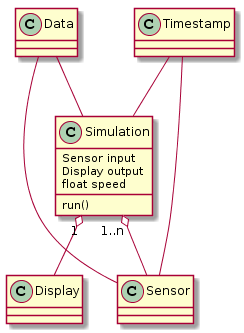
\includegraphics[scale = 0.5]{figures/meta-meta-model.png}
  \label{meta-meta-model}
  \caption{The general model}
\end{figure}

\subsection{Simulation}

The simulation is the core class that will run the simulation. In this class,
the user should be able to define the speed at with he wants to run the
simulation (for example run a simulation twice as fast as it should be). He
will also define the sensors that will be used, and the display where whe wants
to output the data.

Once the different components of the model are given, the user may start the
simulation. The \emph{Simulation} class will then handle time, ask the sensors
for data, and send it to the given display.

\subsection{Display}

This class will deal with the output of the simulation. Many different outputs
can be defined: CSV, JSON formats, or outputing in an influxDB database (that
can be then visualised with Grafana).

The Display is plugged to the simulation and will receive the generated data
as soon as they are generated during the simulation.


\subsection{Sensor}

This is the most base class that will allow the user to define sensors. The
model provides different kinds of predefined Sensors in order to help the user
to easily build their simulation.

Even if different kinds of sensors exist, they must all behave the same
way. Because of this, the Simulation does not have to know what kind of sensors
it is handling.

\subsection{Generator}

Some sensors may be complex to build. If they are an aggregation of many
sensors, or implement complex functions. In order to provide an easy way to
build complex sensors, we made this Generator class. It can be seen as a Sensor
in construction. The user will progressively give data to the Constructor, give
it all the information it needs, and when all options are given, the Generator
will output a Sensor behaving like the user wants.

This is why it is important for all Sensors to behave the same way : the user
does not care how the Sensor behaves internaly, the important information is
the data output. Generators are here to help build Sensors. But they are not
mandatory, the user can build the sensors by hand.

\subsection{Timestamp}

The Timestamp class is here to provide a more friendly interface for
time. There are different kinds of times : absolute dates, relative dates,
durations, ... In order to provide a clean access to all these possibilities,
the Timestamp class tries to overload all basic operations so that time can
be smoothly used in user-defined functions. For example, when one wants a
"function that is a second order polynomial in time", is time an absolute
time (total seconds since Epoch) ? Is it time elapsed since the begining of
the simulation ? Is it a function of the "hour" field of a date ?

The Timestamp allows to access all these informations and use them smoothly.

\subsection{Data}

The Data class will represent a point of data generated by a sensor. It
encapsulates all informations that are needed to describe a piece of
information. It contains the Timestamp when this data was generated, the name
of the sensor that generated it, the value of the data, and all other field
that may be used to describe the data.

This class will not be used by the user but it will be necessary for the
simulation.
